% !TEX root = ../thesis.tex
%\chapter{State of the Art}
\chapter{Ethical Preliminaries}
\label{capitolo2}
\thispagestyle{empty}

\iffalse

This chapter discusses the state of the art that is relevant for your own work. What does that mean? It means that it provides the reader with all the relevant references he/she may need to know in order to understand better three things: (i) the context of your work, (ii) the problem and the need for a solution, and (iii) the value of your contribution. You achieve this by citing works or scientific papers that solved the same or similar problems in the past. Citing does not just mean adding a references to the bibliography and printing a number here; it means you tell the reader about the merits and possible demerits of each of the references you feel relevant. Of course, doing so requires you to first read each reference and, most importantly, to understand it. There should be lots of references in this chapter. 

It is advisable that you structure the chapter into sections in function of the topics you treat. If you do so, before starting with the first section of the chapter, explain the reader how you structure your discussion in one paragraph.

\begin{itemize}
\item[\Square] \emph{Read} relevant literature and or \emph{test} related software or tools.
\item[\Square] \emph{Summarize} your reading.
\item[\Square] Provide correct \emph{references} (the bibliography in the end of this document).
\end{itemize}

\fi


The aim of this chapter is to provide to the reader preliminary notions of ethical and sociological rather than technical nature.

Starting from the concept of \textit{bias}, passing through \textit{discrimination} and \textit{human rights}, we will discuss about \textit{equality}, \textit{equity} and finally \textit{fairness}, by providing definitions and relevant examples from the literature on these topics. Because of the ``dual nature'' of this research, this chapter has to be seen as complementary to the next one, in which some technical bases will be provided, together with an overview on the tools adopted.


\section{Bias}
Although the word ``\textbf{bias}'' doesn't have an intrinsically negative meaning (it is informally used to indicate a deviation from neutrality), it is mostly adopted in contexts where it entails a moral dimension. As reported in \cite[p.332]{friedman2017bias}, \emph{we use the term bias to refer to computer systems that \textit{systematically} and \textit{unfairly discriminate} against certain individuals or groups of individuals in favor of others. A system discriminates unfairly if it denies an opportunity or a good or if it assigns an undesirable outcome to an individual or group of individuals on grounds that are unreasonable or inappropriate}. Therefore, it is important to underline that unfair discrimination due to bias is strictly related to systematic and unfair outcome.

By following the classification provided in \cite{friedman2017bias}, we can distinguish three overarching categories of bias:
\begin{itemize}
\item \textbf{Preexisting bias}: it has its roots in social institutions, practices and attitudes. Preexisting bias may originate in the society at large, in subcultures and organizations, and can enter a computer system either voluntarily or implicitly and unconsciously, even in spite of the best intentions of the system designer.
\item \textbf{Technical bias}: it arises from the resolution of issues in the technical design. Technical bias may originate from design choices, constraints and technological tools, or exacerbate preexisting bias.
\item \textbf{Emerging bias}: it emerges some time after a design is completed, as a result of changing societal knowledge, population, or cultural values. Emerging bias is strictly related to a context of use, and it is the most difficult to detect.
\end{itemize}

For the purpose of this research, we will focus on preexisting bias (in particular, \textit{societal bias}) and technical bias, but it is important to point out that emerging bias shouldn't be underestimated in the long run, especially when it arises from a \textit{mismatch between users and system design} due to \textit{different values}, that is bias originated when a computer system is used by a population with different values than those assumed in the design, because society is in constant change and systems should be readjusted or reinvented in order to keep up with the present.

A significant example of bias is provided in \cite{angwin2016machine}: a commercial tool called COMPAS (Correctional Offender Management Profiling for Alternative Sanctions) was used in courts in the U.S. to automatically predict some categories of future crime to assist in bail and sentencing decisions. On average, the tool correctly predicted recidivism 61\% of the time, but blacks were almost twice as likely as whites to be labeled a higher risk but not actually re-offend. The tool made the opposite mistake among whites: they were much more likely than blacks to be labeled lower risk but go on to commit other crimes.

Other examples, related to gender bias, are given by \cite{gibbs2015women} and \cite{dastin2018amazon}. The former is about a research conducted in 2015, in which a tool was used to simulate job seekers that did not differ in browsing behavior, preferences or demographic characteristics, except in gender. One experiment showed that Google displayed adverts for a career coaching service for ``\$200k+'' executive jobs 1,852 times to the male group and only 318 times to the female group. The latter concerns another Big Tech company, Amazon, whose machine-learning's specialists, back in 2015, discovered that their new recruiting engine was not rating candidates in a gender-neutral way, because the system taught itself that male candidates were preferable by penalizing resumes that included the word ``women's''.


\section{Discrimination}
Bias can lead to \textbf{discrimination}, but what discrimination is and how it occurs is a controversial issue. As reported in \cite{scantamburlo2018machine}, often the law, rather than providing a definition of discrimination, defines a list of attributes, called \textbf{protected attributes}, that cannot be used to take decisions in various settings. The list is non-exhaustive and includes characteristics such as race, sex, religion or sexual orientation. Groups of people characterized by these attributes are therefore classified as \textit{protected groups}. Trying to formalize a bit more, we can define discrimination as the result of:
\begin{itemize}
\item \textbf{Disparate treatment}: the illegal practice of treating an entity, such as a job applicant or an employee, differently based on a protected characteristic such as race, gender, age, religion, sexual orientation, or national origin.
\item \textbf{Disparate impact}: the result of systematic disparate treatment, where disproportionate adverse impact is observed on members of a protected class.
\end{itemize}

On a more sociological perspective, discrimination is strictly related to \textit{human rights} and \textit{equality}.


\section{Human Rights}
For what concerns \textbf{human rights}, there is a lot of debate on how to incorporate them in computer systems by following a ``human-rights-by-design'' approach \cite{penney2018advancing}, in order to contrast the negative effects of the so called ``dual-use technologies'': products which may serve legitimate societal objectives but are also used to undermine human rights like freedom of expression or privacy. Of course, to reach the goal it would require a culture shift and huge efforts from both national governments and businesses, in order to let them design tools, technologies and services to respect human rights by default, rather than permit abuse or exploitation of them.
A similar concept is purposed in \cite{yeung2020ai}, where the authors sketch the contours of a comprehensive governance framework for ensuring AI systems to be ethical in their design, development and deployment, and not violate human rights. This framework should be effective in contrasting \textit{ethics washing}: the practice of fabricating or exaggerating a company's interest in equitable AI systems that work for everyone, a sort of side door that companies use to substitute regulation with ethics.
For the purpose of this research, we can define human rights as \emph{inalienable fundamental rights to which a person is inherently entitled simply because she or he is a human being} \cite[p.3]{sepuldeva2010human}. These norms are concerning every human being, regardless of sex, age, language, religion, ethnicity or any other status.


\section{Equality \& Equity}
Equality is generally intended as \emph{an ideal of uniformity in treatment or status by those in a position to affect either} \cite{britannica2009equality}. The concept of equality is often associated with discrimination mostly because of the article 7 of the Universal Declaration of Human Rights (UDHR), which states: \emph{``All are equal before the law and are entitled without any discrimination to equal protection of the law''} \cite[p.2]{assembly1948universal}. This principle is known as ``equality before the law'', and establishes that everyone must be treated equally under the law regardless of race, gender, color, ethnicity, religion, disability, or other characteristics, without privilege, discrimination or bias.
However, it is important to distinguish between two different political and social theories:
\begin{itemize}
\item \textbf{Equality of opportunity}: \emph{the idea that people ought to be able to compete on equal terms, or on a ``level playing field'', for advantaged offices and positions} \cite{britannica2019equal}. This principle is based on the notion of \textit{sameness}, where fairness is achieved through equal treatment regardless of people's needs. Equality of opportunity is usually simply referred as \textbf{equality}, and from now on we will adopt the same terminology for this research.
\item \textbf{Equality of outcome}: the idea that people should have access to resources (possibly of a different nature and to a different extent) in order to be able to reach the same condition. This principle is based on the notion of \textit{need}, where fairness is achieved by treating people differently depending on their endowments and necessities. Equality of outcome is also known as \textbf{equity}, and from now on we will adopt the same terminology for this research.
\end{itemize}

\begin{figure}[h!]
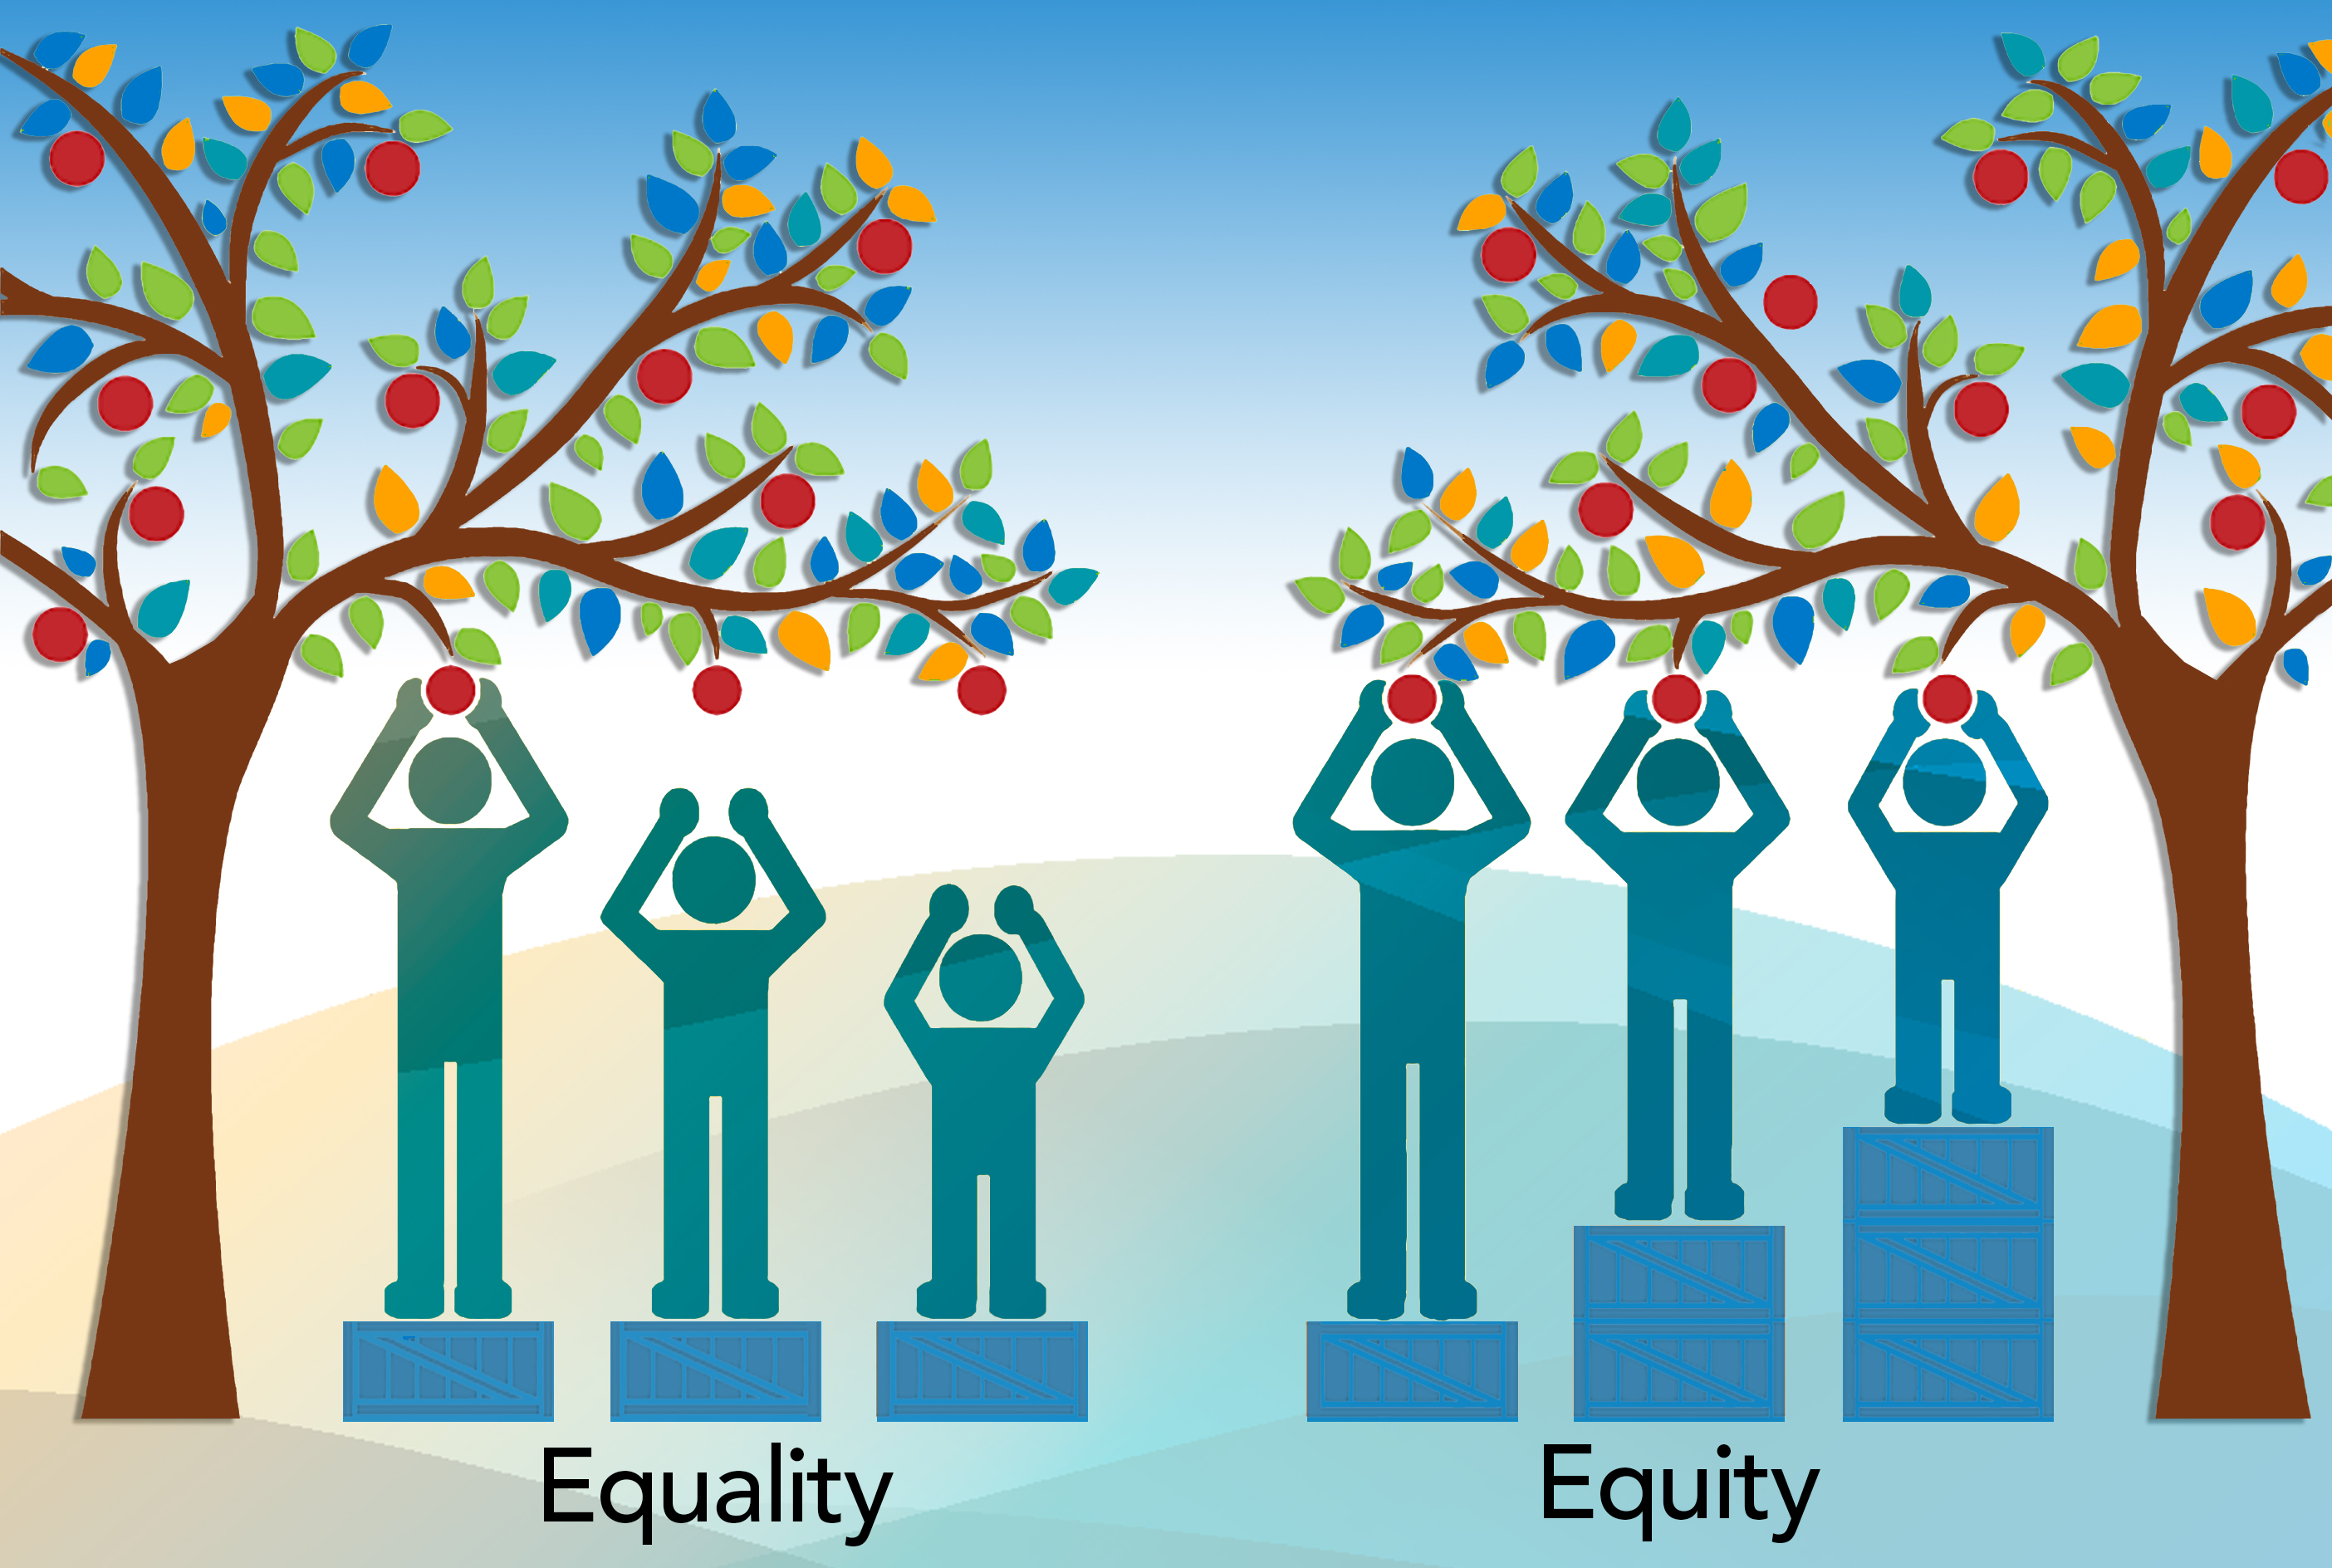
\includegraphics[scale=.5]{figures/equality_vs_equity.jpg}
\centering
\caption{Visual example of the difference between equality and equity.\newline
\copyright 2014, Saskatoon Health Region. Source: \protect\url{https://www.nwhu.on.ca/ourservices/Pages/Equity-vs-Equality.aspx}}
\label{fig:equality_vs_equity}
\end{figure}

Figure \ref{fig:equality_vs_equity} provides a simple example of the difference between equality and equity. Treating people equally, in this scenario, means to give everyone the same one box to reach the fruit, while treating people equitably means to give them as many boxes as they need to achieve the goal. It is important to notice that equity could require (and often requires) unequal treatment.

The authors of \cite{jagadish2021facets} distinguish between four different facets of data equity (which, as the name itself suggest, is an extension of the equity concept in the technical context of data systems):
\begin{itemize}
\item \textbf{Representation equity}: bias may arise because of material deviations between the data and the world represented by the data, often with respect to historically disadvantaged and underrepresented groups. Even when dealing with contemporary data, disparities rooted in historical discrimination can lead to representation inequities and therefore to the introduction or the exacerbation of problems. For example, in the U.S. there has been a lot of discussion about racial disparities concerning COVID-19, regarding both availability of testing (fewer test sites in minorities neighborhoods, historically poorer) and desire of individuals to be tested (black people more suspicious about the medical system, because of their history of unfair treatments). Another example is related to Amazon and a software developed by the company for screening candidates for employment: the software was trained on the already hired employees and since they were mostly males, females became underrepresented in the data and the software was much more likely to mark women as unsuitable for hiring.
\item \textbf{Feature equity}: bias may arise because not all the features needed to represent a marginalized group of people and required for a particular analysis are available in the data. As an example, for a specific study involving transgender people may be important to distinguish between their birth name and their self-assigned name.
\item \textbf{Access equity}: bias may arise because of a not equitable and partecipatory access to data and data products across domains and levels of expertise, or even because of the opacity of data systems.
\item \textbf{Outcome equity}: bias may arise because of a lack of monitoring and mitigation of unintended consequences for any group affected by the system after deployment, directly or indirectly (for example, contact tracing apps may facilitate stigma or harassment).
\end{itemize}


\section{Fairness}
As discussed in the previous section, both equality and equity aim to achieve \textbf{fairness}, despite the different approaches of the two philosophies. We can therefore distinguish between two different concepts of fairness \cite{dwork2012fairness}:
\begin{itemize}
\item \textbf{Individual fairness}: any two individuals who are similar \textit{with respect to a task} should receive similar outcomes. The similarity between individuals should be captured by an appropriate metric function, usually difficult to determine. Individual fairness is strictly related to the idea of equality.
\item \textbf{Group fairness} (also known as \textit{statistical parity}): demographics of the individuals receiving any outcome - positive or negative - should be the same as demographics of the underlying population. Group fairness equalizes outcomes across protected and non-protected groups, and is therefore strictly related to the idea of equity.
\end{itemize}

Despite individual and group fairness are not mutually exclusive in theory, in real life it is often hard to conciliate the two approaches. Furthermore, this categorization is not the only possible one: the authors of \cite{verma2018fairness} collected and provided about twenty among the most prominent definitions of fairness, and applied each of them to a case study based on gender-related discrimination, in which the aim was to assign a credit score to people requesting a loan by using ``Personal status and gender'' as a protected attribute for the decision-making process.

Among the others, a couple of peculiar definitions, often listed together with individual and group fairness, are the following:
\begin{itemize}
\item \textbf{Fairness through unawareness}: protected attributes are not used in the decision-making process, and therefore the subsequent decisions cannot rely on them. This ``blind'' approach relies on \textit{impartiality} and is consistent with the disparate treatment principle, but removing features means losing information, and furthermore there could be features correlated to protected attributes that would not be removed, potentially introducing bias.
\item \textbf{Counterfactual fairness}: a precise and non-technical definition is provided in \cite[p.1]{wu2019counterfactual}: \emph{a model is fair if for a particular individual or group its prediction in the real world is the same as that in the counterfactual world where the individual(s) had belonged to a different demographic group. However, an inherent limitation of counterfactual fairness is that it cannot be uniquely quantified from the observational data in certain situations, due to the unidentifiability of the counterfactual quantity}.
\end{itemize}

The classifier resulted to be fair depending on the notion of fairness adopted, showing the impossibility of addressing fairness as a unique, broad and inseparable concept. This result is coherent with \textit{Chouldechova's impossibility theorem} \cite{chouldechova2017fair}, which demonstrates, taking three definitions of fairness, the impossibility of satisfying all of them.


\iffalse

Fairness requires social consensus.
Humans have many biases, no human is perfectly fair, even with the best of intentions.
Bias in algorithms in easier to detect than human bias, because humans are likely to defend their decisions with plausible explanations.
In machine learning, the past is assumed to be representative of the future (training, test); but in society this is often not true, because the world continuously change.

\textbf{Stability}: if you choose a different model, how likely is it that a small perturbation will result in a different answer?


\section{Summary}
Close the state of the art chapter with some words that connect the discussion of the references to your thesis. Pay attention that the reader understands why you discussed the works/topics you discussed and how they are related to what you do.

\begin{itemize}
\item[\Square] Show that in the state of the art the \emph{problem} you want to solve has not yet been solved or not been solved in an as efficient / effective / easy to use / cost-saving fashion as you target with your work.
\item[\Square] If your work has similarities with some \emph{specific references}, point them out here and explain why these are particularly important to you. Perhaps you started your investigation from the outputs of a specific paper or you want to improve the performance of an algorithm studied earlier; it's good to mention this here.
\item[\Square] Attention: this is not yet the place where to anticipate \emph{your solution}. You may give hints, but it's too early to make a comparison between your work and the state of the art, as the reader does not yet know anything about your work. This discussion can go into the final chapter.
\end{itemize}

\fi
